\documentclass[a4paper,12pt]{article} 

%%% Работа с русским языком
\usepackage{cmap}                           % поиск в PDF
\usepackage{mathtext} 			 	       % русские буквы в формулах
\usepackage[T2A]{fontenc}               % кодировка
\usepackage[utf8]{inputenc}              % кодировка исходного текста
\usepackage[english,russian]{babel}  % локализация и переносы

%Матеша
\usepackage{amsmath,amsfonts,amssymb,amsthm,mathtools} % AMS
\usepackage{icomma} % "Умная" запятая

\usepackage{gensymb}

%\mathtoolsset{showonlyrefs=true} % Показывать номера только у тех формул, на которые есть \eqref{} в тексте.

%% Шрифты
\usepackage{euscript}	 % Шрифт Евклид
\usepackage{mathrsfs} % Красивый матшрифт


\usepackage[utf8]{inputenc}
\usepackage[russian]{babel}
\usepackage[OT1]{fontenc}
\usepackage{amsmath}
\usepackage{amsfonts}
\usepackage{amssymb}
\usepackage{graphicx}
\usepackage[left=2cm,right=2cm,top=2cm,bottom=2cm]{geometry}
\usepackage{calc}
\usepackage{wrapfig}
\usepackage{setspace}
\usepackage{indentfirst}


%% Свои команды
\DeclareMathOperator{\sgn}{\mathop{sgn}}

%% Перенос знаков в формулах (по Львовскому)
\newcommand*{\hm}[1]{#1\nobreak\discretionary{}
{\hbox{$\mathsurround=0pt #1$}}{}}

%%% Заголовок
\author{Злобина Вера}
\title{Лабораторная работа 1.1.6

Изучение электронного осциллографа}

\begin{document} 	
	
	
	
	\maketitle
	
	\newpage
	
	
	\subparagraph*{Цель работы:} ознакомление с устройством и работой осциллографа и изучение его основных характеристик.
	
	
	\subparagraph*{В работе используются:} осциллограф, генераторы электрических сигналов, соединительные кабели.
	
	\section*{Теоретические сведения}
	
	Осциллограф -- регистрирующий прибор, в котором исследуемый сигнал преобразуется в видимый на экране график изменения напряжения от времени. Осциллограф широко используется в физическом эксперименте, так как с его помощью можно регестрировать любую величину, которую можно преобразовать в электрический сигнал.
	\subsection*{Устройство осциллографа}

	

		\begin{center}
			\begin{tabular}{c}
			
			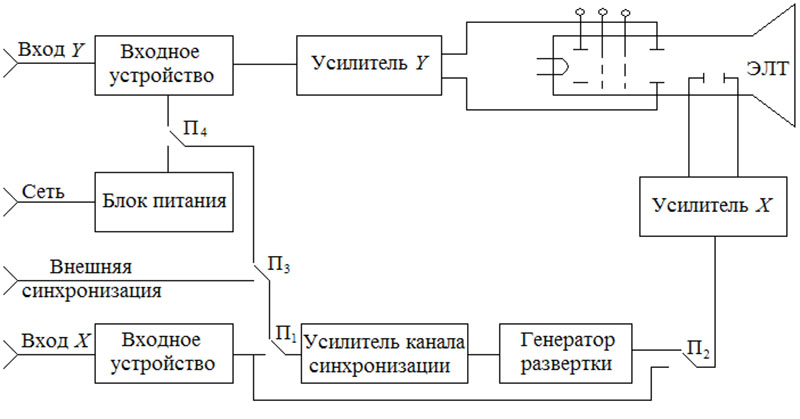
\includegraphics[width=0.7\linewidth]{pic1.jpg}\\
		\\	Cхема устройства осциллографа
	
	\end{tabular}
		\end{center}

	
	
	
	\subsection*{Принцип работы}
	Основной элесент осциллографа -- электронно-лучевая трубка. Электронный пучок формируется системой электродов, называемой электронной пушкой: катод с нагревателем, модулятор, фокусирующий и ускоряющий аноды. Форма, размеры и расположение электродов подобраны таким образом, чтобы разгонять электроны и фокусировать пучок на экране. 
	
	На пути к экрану, сформированный пучок проходит две пары отклоняющих пластин. Две вертикальные пластины образуют плоский конденсатор, поле которого способно отклонять пучок в горизонтальном направлении. Аналогично, поле горизонтального конденсатора способно отклонять пучок в вертикальном направлении. Подавая на пластины электрическое напряжение и отслеживая траеторию пучка на экране можно анализировать входящий сигнал.
	
	\textbf{Развертка}
	
	Так как подаваемые на пластины сигналы лежат в довольно широком диапазоне, а чувствительность трубки довольно сильно ограничена, то в конструкции осциллографа присутствуют делители и усилетели.
	
	Для получения на экране изображения необходимо выполнение двух условий:
	
	\begin{enumerate}
		\item Подаваемое на вертикально отклоняющие пластины напряжение должно линейно завсить от сигнала.
		\item Подаваемое на горизонтально отклоняющие пластины напряжение должно линейно зависить от времени.
	\end{enumerate}
	
	В таком случае, напряжение пилообразной формы, вырабатываемое генератором, (Которое называется напряжением развертки) имеет вид, представленный на рисунке .
	
	


		\begin{center}
	\begin{tabular}{c}
		
		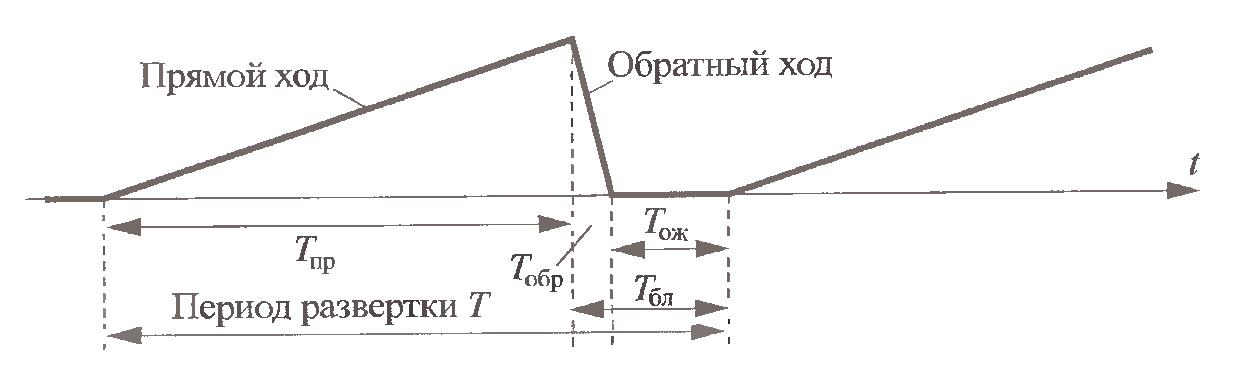
\includegraphics[width=0.7\linewidth]{pic3.jpg}\\
		\\	Напряжение развёртки
		
	\end{tabular}
\end{center}
	
	Кроме того, еще один важный процесс - синхронизация. Для получения устойчивой картины сигнала на экране необходимо, чтобы период развертки был кратен периоду самого сигнала.
	


\begin{center}
	\begin{tabular}{c}
		
		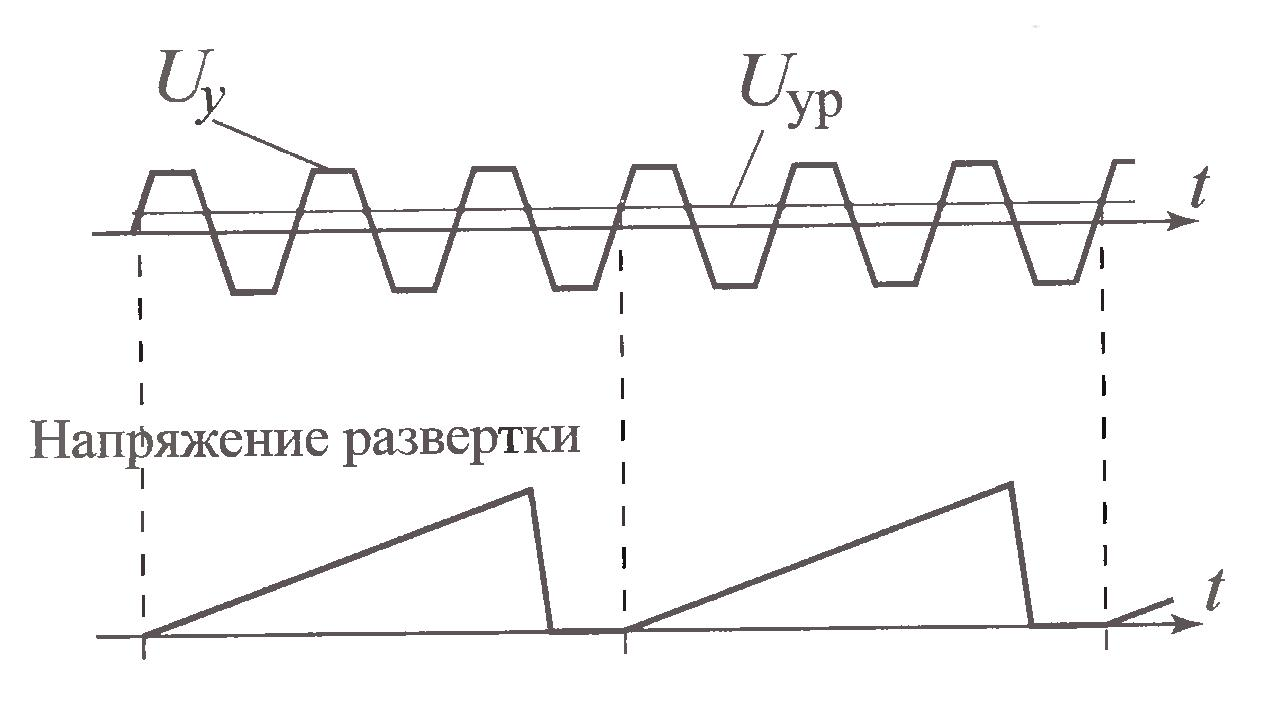
\includegraphics[width=0.7\linewidth]{pic2.jpg}\\
		\\	Условие наблюдения устойчивой картины сигнала на экране осциллографа
		
	\end{tabular}
\end{center}

\newpage

	\subsection*{Наблюдение периодического сигнала от генератора и измерение его частоты.}
\begin{table}[h!]
	\begin{center}
	\begin{tabular}{|l|l|l|l|l|l|l|}
		\hline
	$	f_{zg}, Гц $& T, дел & time/div & T, с     & f, Гц           & df, Гц         & f - fzg, Гц \\ \hline
		1999  & 5      &   $10^{-4}$& 0,0005   & 2000            & 80             & 1           \\ \hline
		1299  & 7,8    & $10^{-4}$ & 0,00078  & 1280& 30 & 19         \\ \hline
		534   & 9,4    & $2 \cdot 10^{-4}$& 0,00188  & 530   & 10& 4        \\ \hline
		2502  & 8      &$ 5 \cdot 10^{-5}$ & 0,0004   & 2500            & 60         & 2         \\ \hline
		4714  & 4,3    &$ 5 \cdot 10^{-5}$  & 0,000215 & 4700 & 200 & 14    \\ \hline
	\end{tabular}
\caption{Период и частота синусоидального сигнала}
\end{center}
\end{table}
	
	\subsection*{Измерение амплитуды сигнала}
	\begin{align*}
	U_{MAX} =& 11В&
	U_{MIN} =& 0.6мВ& \\
	2.2дел;\: \: & 5\frac{В}{дел}&
	2.4дел;\: \: & 5\frac{мВ}{дел}& \\
	\frac{\delta U_{MAX}}{U_{MAX}} \approx& 0.05& 
	\frac{\delta U_{MIN}}{U_{MIN}} \approx& 0.08& 
	\end{align*}
	
	
	
	\begin{equation*}
	\beta_{21}[дБ]=10\lg\frac{P_2}{P_1}=20\lg\frac{U_2}{U_1}=25.3дБ \: \: \: \: \delta \beta_{21} \approx 0.1
	\end{equation*}
	
	где $P_2/P_1$ — отношение средних мощностей, $U_2/U_1$ — отношениеамплитуд некоторых двух сигналов (здесь учтено, что мощностьпопорциональна квадрату амплитуды $P \sim U^2$).
	
%	\newpage
	
	\subsection*{Измерение амплитудно-частотной характеристики осциллографа}
	
	Измерим амплитудно-частотную характеристику K(f) при открытом (DC,$\:\approx$) и при закрытом (AC,$\:\sim$) входе. Результаты занесeм в таблицу.
	
	\begin{table}[h!]
		\centering
		\begin{tabular}{|c |c|c |c|c|c|}
			\hline
			$f_{ген}$ & $\lg f$ & $U_{AC}, ДЕЛ$& $K_{AC}$&$U_{DC}, ДЕЛ$& $K_{DC}$ \\
			\hline
			1 & 0.0 & 1.6 & 0.32 & 5.0 & 1.00 \\
			3 & 0.5 & 3.2 & 0.64 & 5.0 & 1.00 \\
			5 & 0.7 & 4.0 & 0.80 & 5.0 & 1.00 \\
			8 & 0.9 & 4.8 & 0.96 & 5.0 & 1.00 \\
			10 & 1.0 & 4.9 & 0.98 & 5.0 & 1.00 \\
			50 & 1.7 & 5.0 & 1.00 & 5.0 & 1.00 \\
			$10^2$ & 2.0 & 5.0 & 1.00 & 5.0 & 1.00 \\
		$10^3$  & 3.0 & 5.0 & 1.00 & 5.0 & 1.00 \\
			$10^6$  & 6.0 & 5.0 & 1.00 & 5.0 & 1.00 \\
			$5 \cdot 10^6$  & 6.7 & 4.8 & 0.96 & 4.8 & 0.96 \\
		$10^7$ & 7.0 & 4.4 & 0.88 & 4.4 & 0.88 \\
			$1.5 \cdot 10^7$  & 7.2 & 4.0 & 0.80 & 4.0 & 0.80 \\
		$2 \cdot 10^7$  & 7.3 & 3.6 & 0.72 & 3.6 & 0.72 \\
			\hline
		\end{tabular}
	\caption{Амплитудно-частотная характеристика}
	\end{table}
	

	
		\begin{center}
	\begin{tabular}{c}
		
		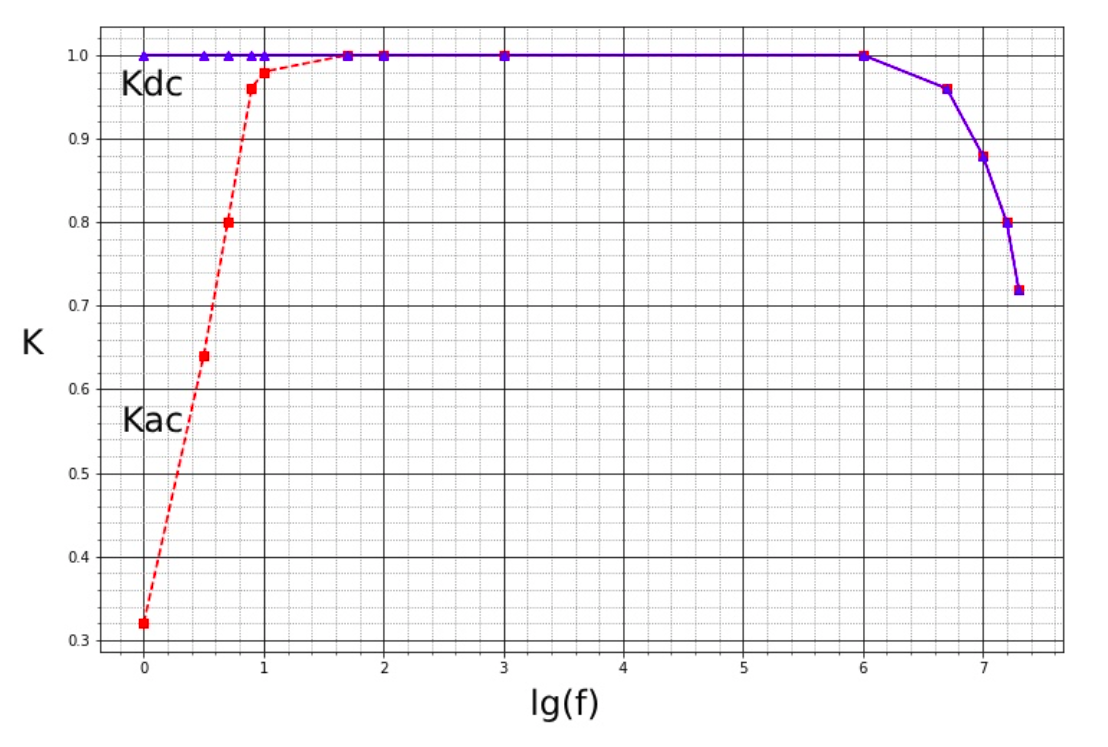
\includegraphics[width=1.0\linewidth]{f5.png}\\
		\\	Зависимость величины $K$ от частоты сигнала
		
	\end{tabular}
\end{center}
%\newpage

	

	\subsection*{Измерение разности фазово-частотных характеристик каналов осциллографа}
	

	
	При подаче на взаимно перпендикулярные отклоняющие пла-стины двух синусоидальных сигналов траектория луча на экранеосциллографа представляет собой эллипс и может быть в общемвиде описана уравнениями:
	
	
	Тогда: 
	\begin{equation*}
	\delta\Phi = arcsin|\frac{y_0}{A_y}| \:\: или \:\: \delta\Phi = \pi - arcsin|\frac{y_0}{A_y}| \:\: или \:\: \delta\Phi = \pi + arcsin|\frac{y_0}{A_y}|
	\end{equation*}


\begin{table}[h!]
	\centering
	\begin{tabular}{|c| c| c| c| c |c |c |c|}
		\hline
	$f_{ген}, Гц$&	10 & $10^3$  & $5 \cdot 10^4$  & $10^5$  & $5 \cdot 10^5$ & $10^6$ & $1.5 \cdot 10^6$  \\ 	\hline
	$\lg f$ &	1.0 & 3.0 & 4.7 & 5.0 & 5.7 & 6.0 & 6.2 \\	\hline
	$2y_0, ДЕЛ$	&0.0 & 0.0 & 0.2 & 0.4 & 1.2 & 2.4 & 3.8 \\	\hline
		$2A_y, ДЕЛ$ &0.0 & 0.0 & 5.0 & 5.0 & 5.0 & 5.0 & 5.0 \\	\hline
		$\Delta\Phi, рад$ &0.00 & 0.00 & 0.04 & 0.08 & 0.24 & 0.50 & 0.86 \\ 	\hline
	\end{tabular}
\caption{Зависимость величины разности фаз от частоты сигнала}
\end{table}

	\begin{center}
	\begin{tabular}{c}
		
	\bfseries{	Зависимость величины разности фаз от частоты сигнала  }\\ 
		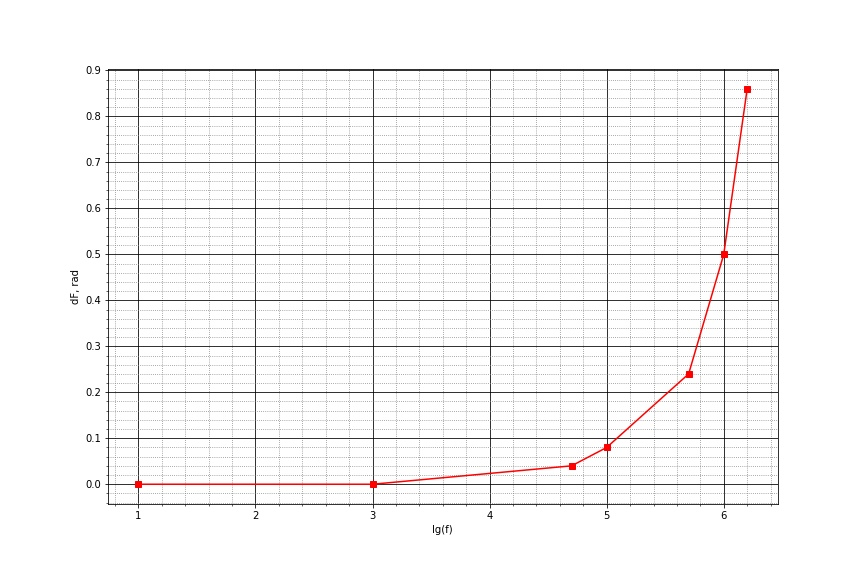
\includegraphics[width=1.0\linewidth]{gr5.jpg}\\
		
	\end{tabular}
\end{center}

Исходя из графика сделаем вывод, что осциллограф отображает корректную разность фаз для $f  < 1кГц$.

%\newpage

	\subsection*{Наблюдение фигур Лиссажу}

		\begin{center}

	
		\begin{tabular}{c c c}
			
			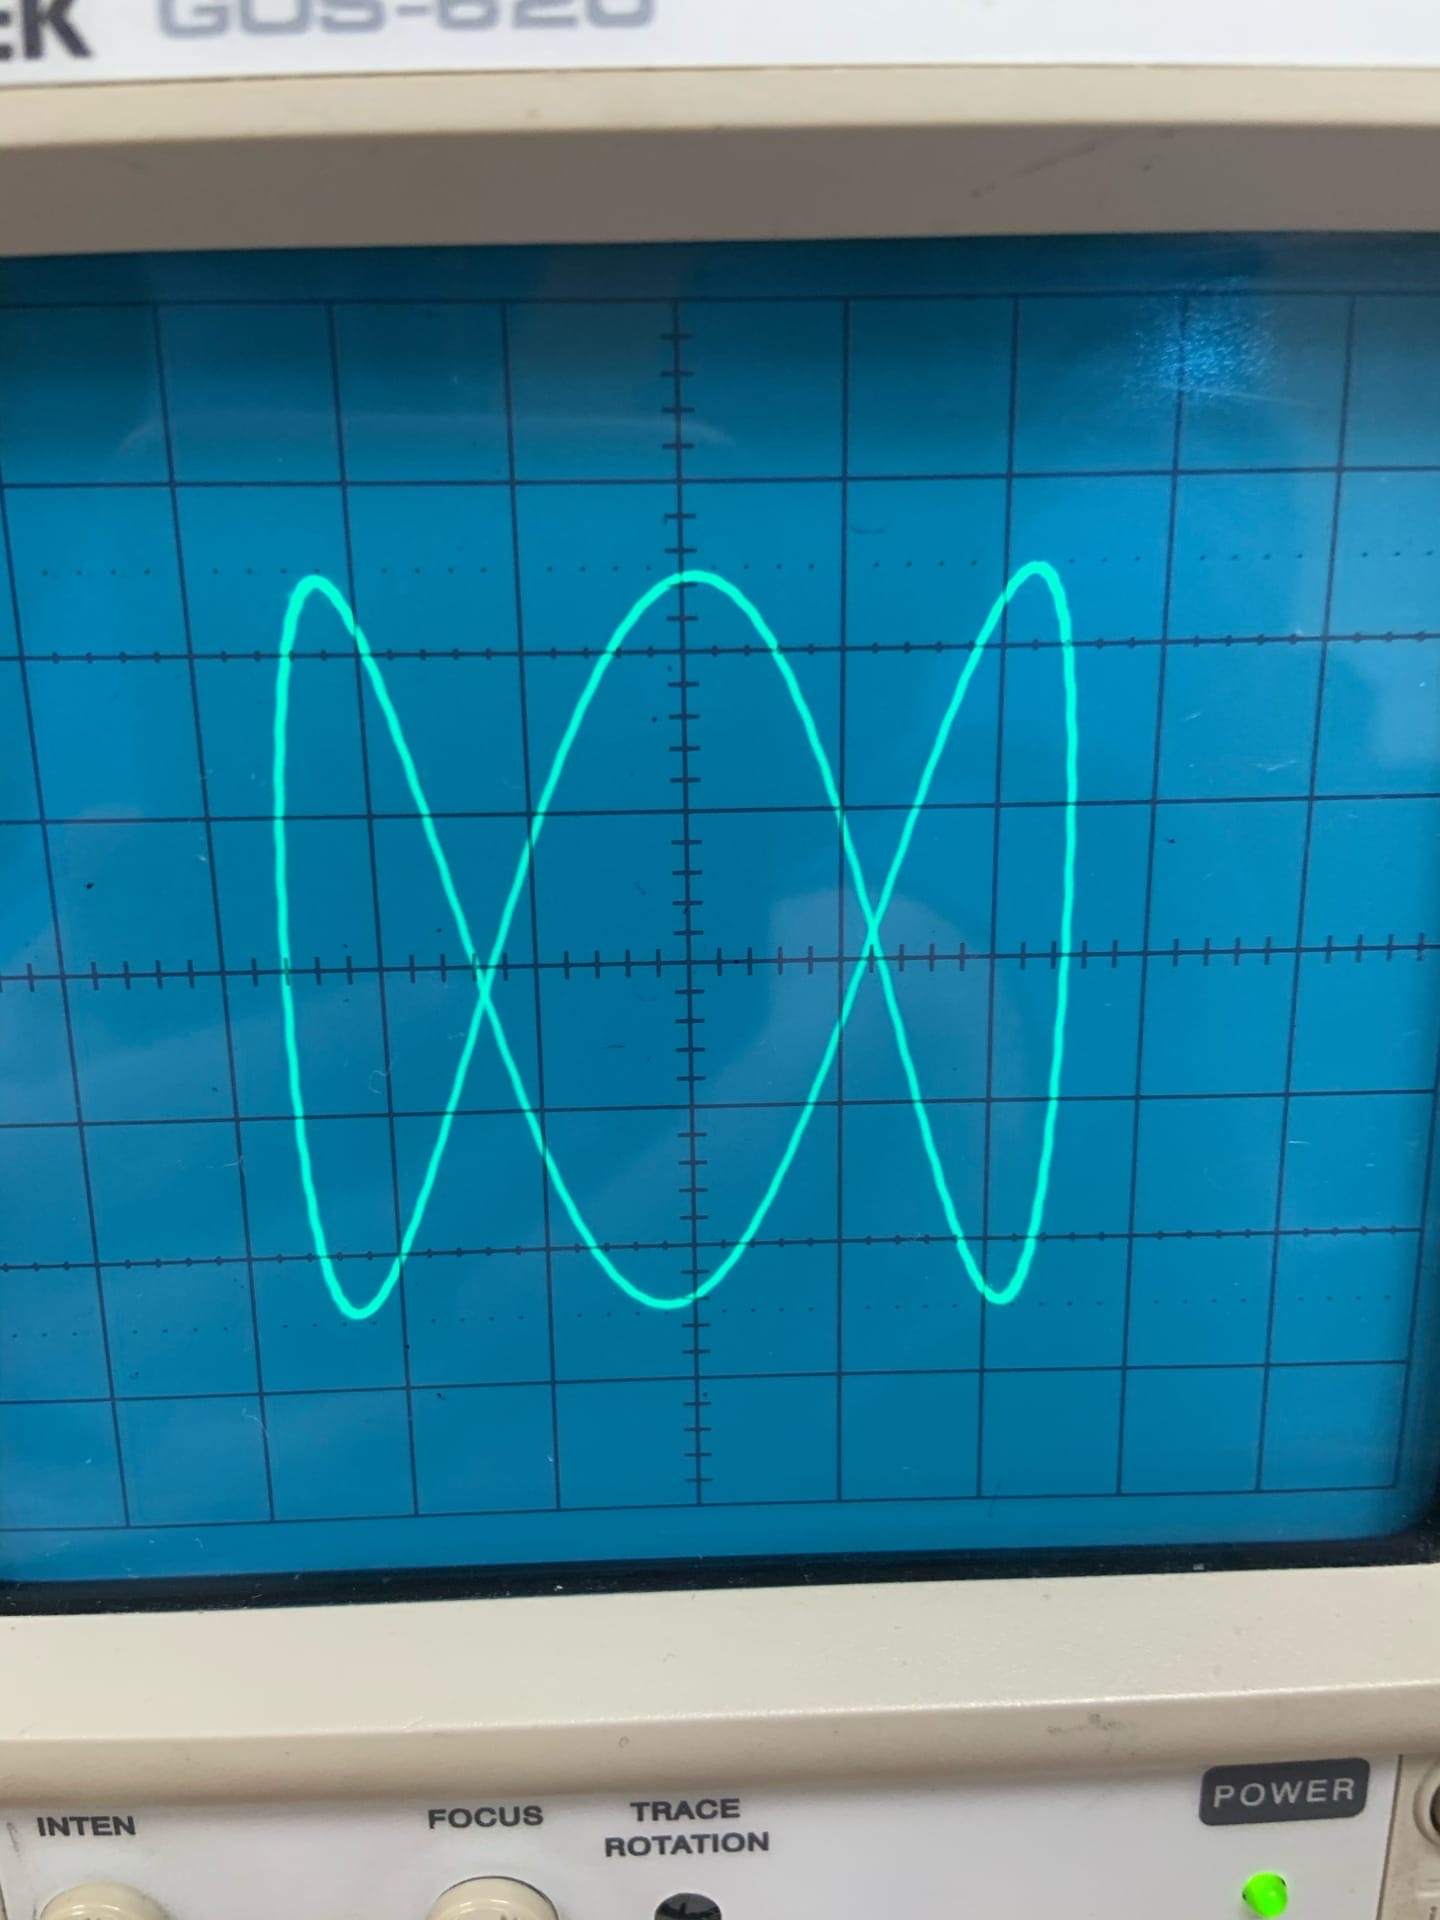
\includegraphics[width=0.3\linewidth]{l1.jpg} & 	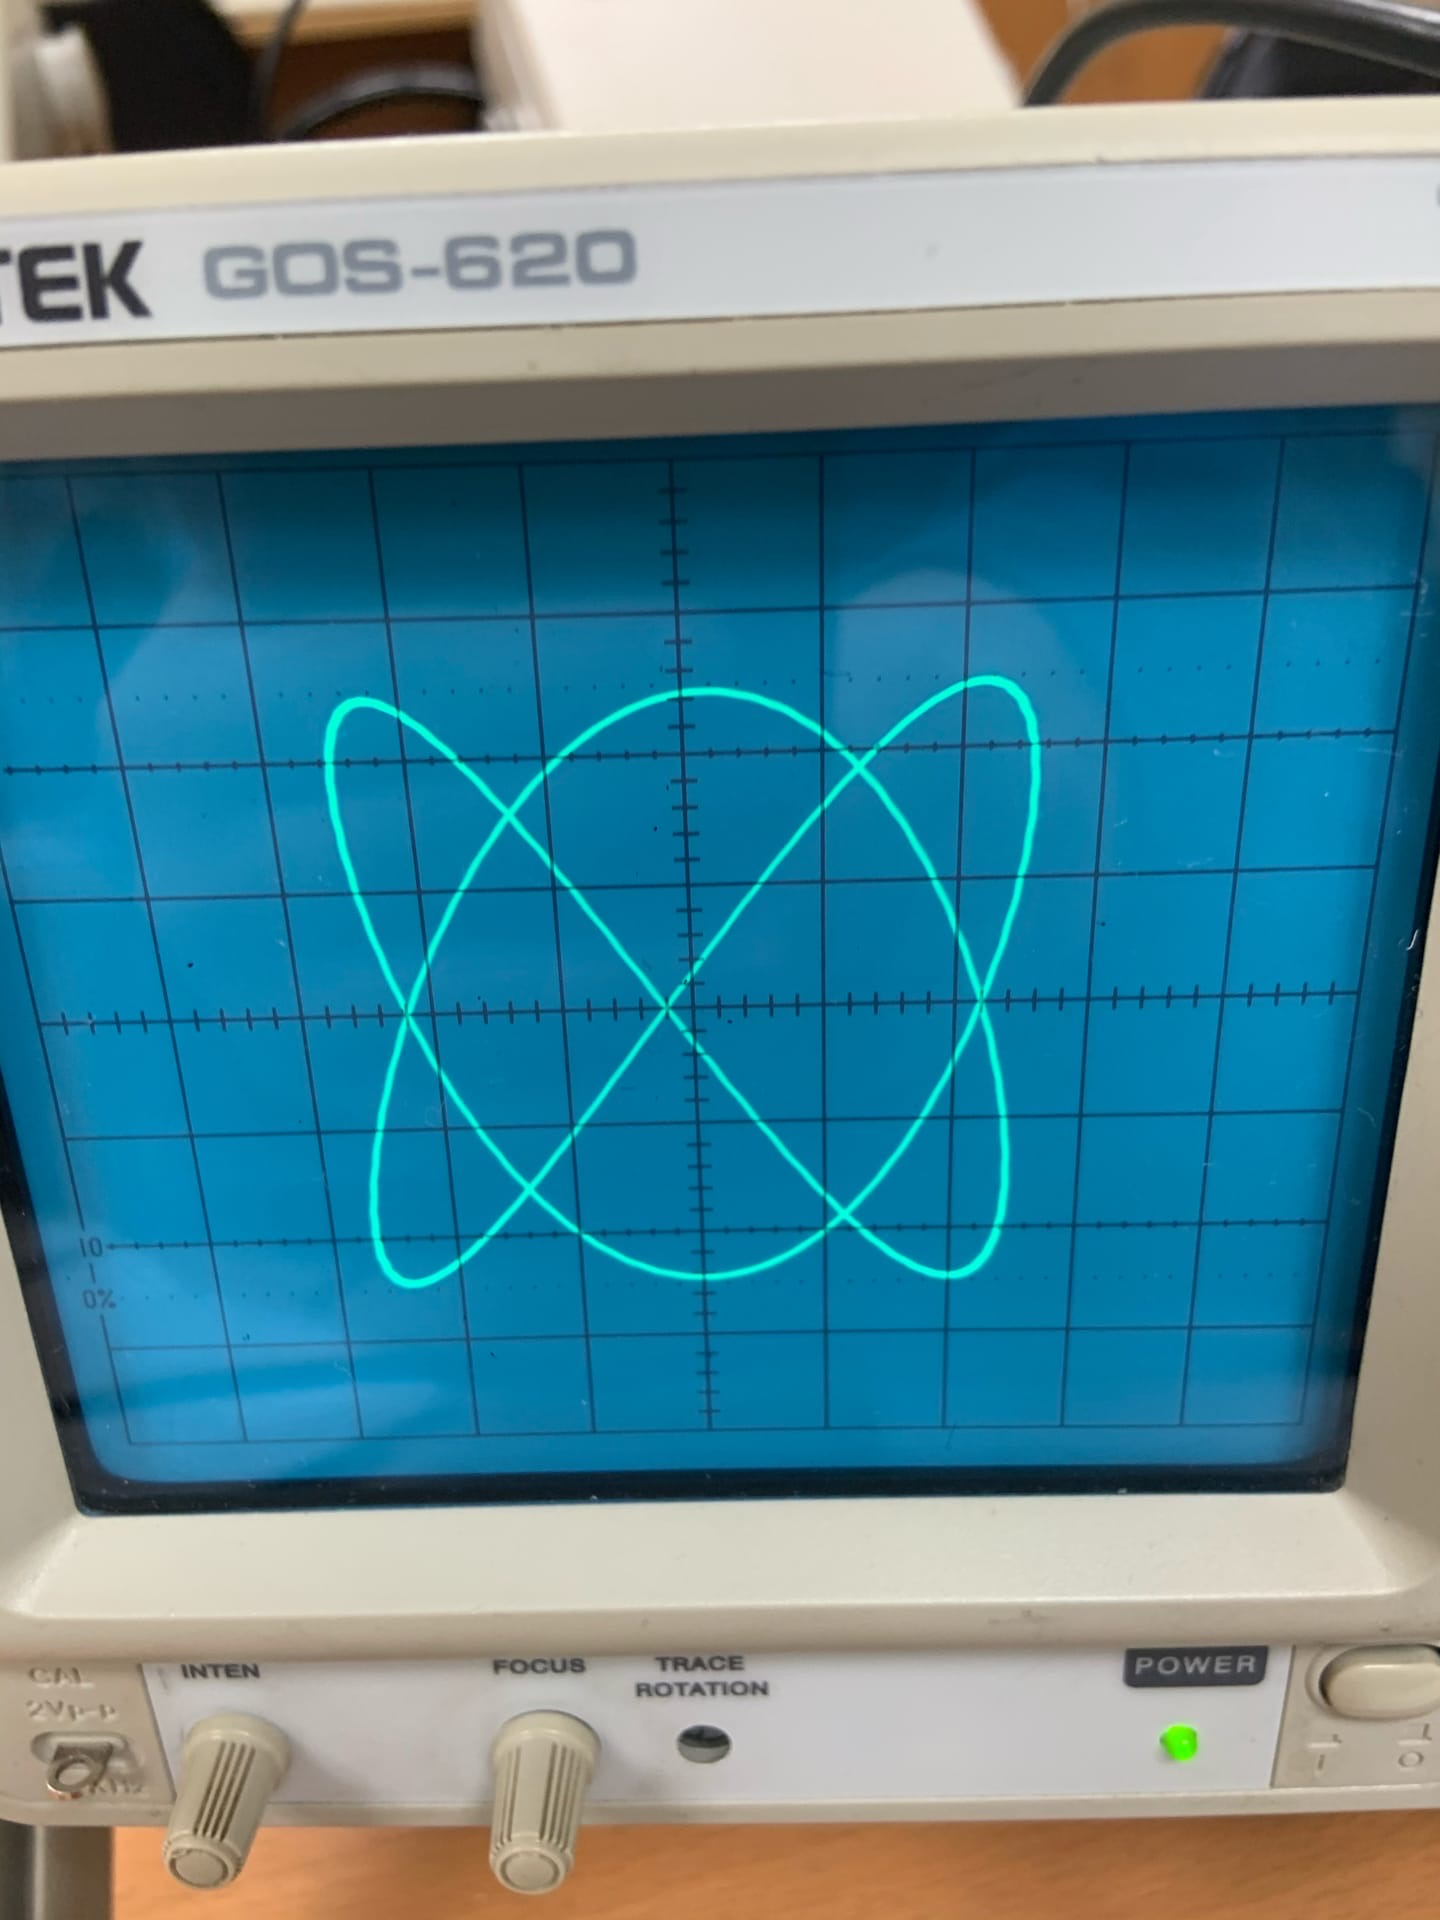
\includegraphics[width=0.3\linewidth]{l2.jpg}& 	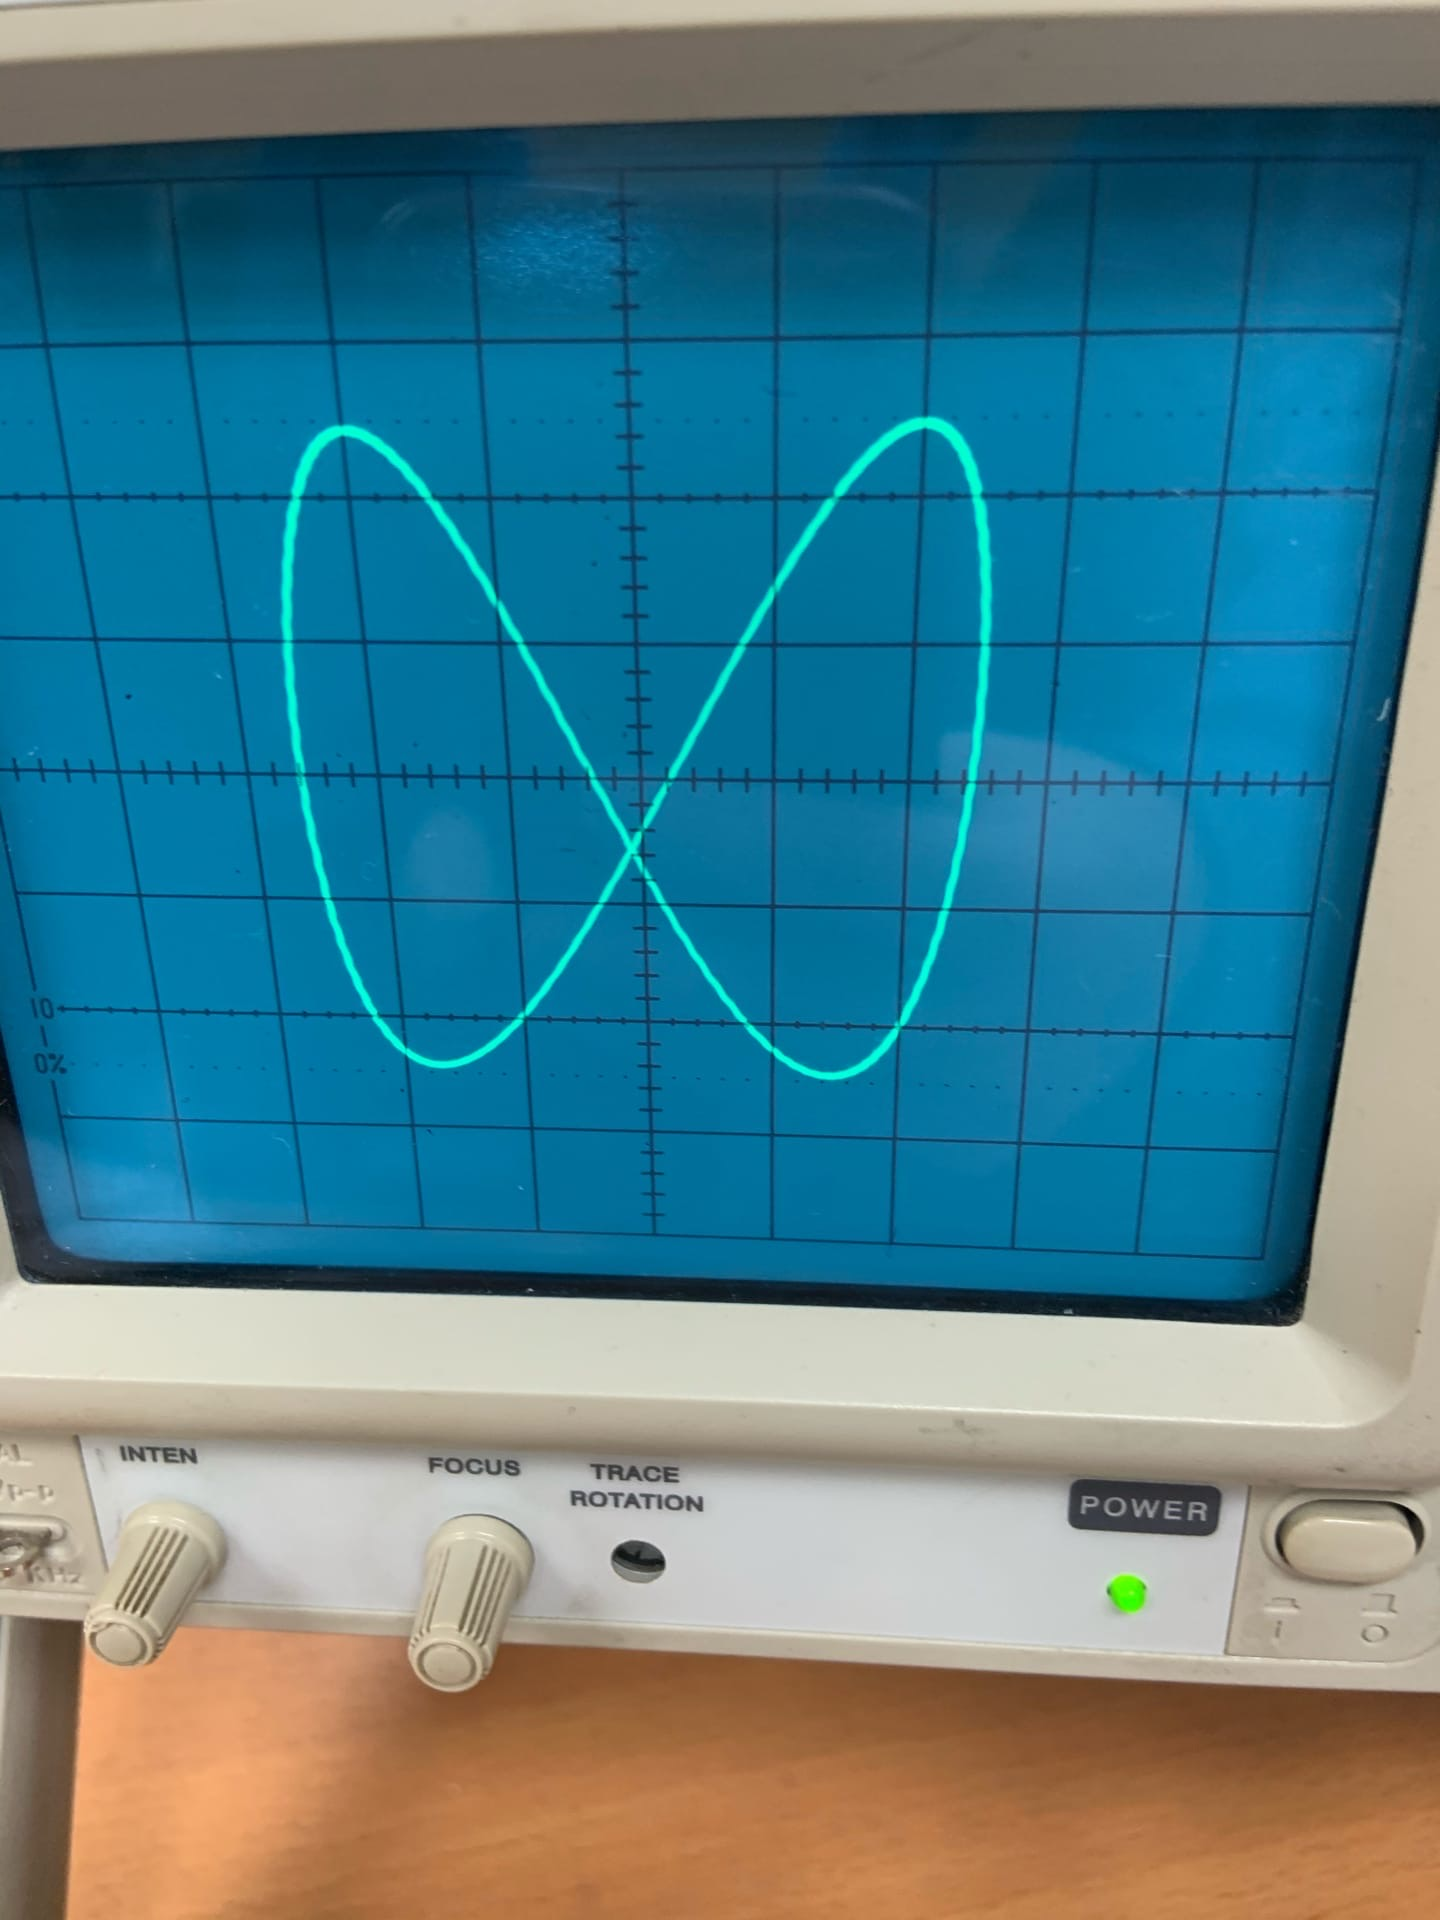
\includegraphics[width=0.3\linewidth]{l3.jpg}\\
			
	
			
\end{tabular} 

Фигуры Лиссажу для соотношения частот 1:3, 2:3 и 1:2 \\ 

	\end{center}


	

	\newpage
	
	
	\section*{Вывод}
В результате работы был изучен электронный осциллограф. Выяснилось, что на больших и низких частотах из-за конструктивных особенностей прибора результаты измерений искажаются. Помимо этого были при помощи осциллографа были получены фигуры Лиссажу.






\newpage



\end{document}